%\iffalse
% pressrelease.dtx generated using makedtx version 1.1 (c) Nicola Talbot
% Command line args:
%   -src "pressrelease.cls\Z=>pressrelease.cls"
%   -src "(.+\.sty)\Z=>\1"
%   -doc "pressrelease-manual.tex"
%   -author "Nicola Talbot"
%   pressrelease
% Created on 2014/9/10 18:01
%\fi
%\iffalse
%<*package>
%% \CharacterTable
%%  {Upper-case    \A\B\C\D\E\F\G\H\I\J\K\L\M\N\O\P\Q\R\S\T\U\V\W\X\Y\Z
%%   Lower-case    \a\b\c\d\e\f\g\h\i\j\k\l\m\n\o\p\q\r\s\t\u\v\w\x\y\z
%%   Digits        \0\1\2\3\4\5\6\7\8\9
%%   Exclamation   \!     Double quote  \"     Hash (number) \#
%%   Dollar        \$     Percent       \%     Ampersand     \&
%%   Acute accent  \'     Left paren    \(     Right paren   \)
%%   Asterisk      \*     Plus          \+     Comma         \,
%%   Minus         \-     Point         \.     Solidus       \/
%%   Colon         \:     Semicolon     \;     Less than     \<
%%   Equals        \=     Greater than  \>     Question mark \?
%%   Commercial at \@     Left bracket  \[     Backslash     \\
%%   Right bracket \]     Circumflex    \^     Underscore    \_
%%   Grave accent  \`     Left brace    \{     Vertical bar  \|
%%   Right brace   \}     Tilde         \~}
%</package>
%\fi
% \iffalse
% Doc-Source file to use with LaTeX2e
% Copyright (C) 2014 Nicola Talbot, all rights reserved.
% \fi
% \iffalse
%<*driver>
\documentclass{nlctdoc}

\usepackage{alltt}
\usepackage{verbatim}
\usepackage{graphicx}
\usepackage[utf8]{inputenc}
\usepackage[T1]{fontenc}
\usepackage[colorlinks,
            bookmarks,
            hyperindex=false,
            pdfauthor={Nicola L.C. Talbot},
            pdftitle={pressrelease.cls: LaTeX class for typesetting press releases},
            pdfkeywords={LaTeX,press release}]{hyperref}


\CheckSum{776}

\newcommand*{\opt}[1]{\csopt{PRset}{#1}}
\providecommand*{\optfmt}[1]{\textsf{#1}}
\renewcommand*{\ienv}[1]{\SpecialEnvIndex{#1}}
\renewcommand*{\usage}[1]{\hyperpage{#1}}
\renewcommand*{\main}[1]{\hyperpage{#1}}
\IndexPrologue{\section*{\indexname}\markboth{\indexname}{\indexname}}
\setcounter{IndexColumns}{2}

\begin{document}
\DocInput{pressrelease.dtx}
\end{document}
%</driver>
%\fi
%
%\MakeShortVerb{"}
%
%\title{pressrelease v1.0:
%typesetting press releases}
%\author{Nicola L. C. Talbot\\\url{http://www.dickimaw-books.com/}}
%
%\date{2014-09-10}
%\maketitle
%
%\begin{abstract}
%The \clsfmt{pressrelease} class is provided for typesetting press
%releases. I wrote it because I found that \cls{newlfm}'s press
%release option wasn't sufficiently configurable for my requirements.
%Sample documents should be available in the \texttt{samples} subdirectory
%of the directory where this document is located.
%\end{abstract}
%
%\tableofcontents
%
%\section{Introduction}
%\label{sec:intro}
%
%A press release is a written statement to inform the media of
%forthcoming events, new products, awards or any other type of news
%item. A press release should be a~compact document that briefly
%outlines the main details of the news item. Therefore press releases
%are usually no longer than a~single page. Hard copies are typically
%double-spaced to allow the journalist room to scribble notes. The
%end of the press release is signalled by three hash (\#) signs
%(\term{end of release marker}).
%
%The \clsfmt{pressrelease} class is loaded in the usual \LaTeX\
%manner:
%\begin{verbatim}
%\documentclass{pressrelease}
%\end{verbatim}
%You may specify the class options: \clsopt{10pt}, \clsopt{11pt},
%\clsopt{12pt}, \clsopt{a4paper}, \clsopt{letterpaper}. These are the
%same as the standard class options of the same names. The
%\sty{geometry} package is automatically loaded so if you want to
%change the page size you can do so using \cs{geometry} (see the
%\sty{geometry} documentation for further details). You can also use
%the class option \clsopt{symbols} to automatically load the
%accompanying \sty{pressrelease-symbols} package (see
%\sectionref{sec:tags}).
%
%Within the \envfmt{document} environment, the contents of the press
%release should be placed inside the \env{pressrelease} environment.
%\begin{definition}[\DescribeEnv{pressrelease}]
%\cs{begin}\{pressrelease\}\newline
%\meta{press release content}\newline
%\cs{end}\{pressrelease\}
%\end{definition}
%
%Within the \env{pressrelease} environment you can use the
%\envfmt{about} environment for information about the company.
%\begin{definition}[\DescribeEnv{about}]
%\cs{begin}\{about\}\newline
%\meta{Information}\newline
%\cs{end}\{about\}
%\end{definition}
%
%The contents of the \env{pressrelease} environment are double-spaced
%(using the \sty{setspace} package, which is loaded by
%default). Two \LaTeX\ runs are required to ensure the last page
%information is correct.
%
%\section{Data Setting Commands}
%\label{sec:datacommands}
%
%In the preamble (or anywhere before the start of the
%\env{pressrelease} environment) you may use the commands described below
%to provide data used in the press release.
%You can later access the information provided using
%\begin{definition}[\DescribeMacro\PRusevar]
%\cs{PRusevar}\marg{variable}
%\end{definition}
%where \meta{variable} is the variable name. For example, to access
%the information provided by \cs{PRcompany}, you can use
%\verb|\PRusevar{company}|.
%
%\begin{definition}[\DescribeMacro\PRheadline]
%\cs{PRheadline}\marg{text}
%\end{definition}
%This specifies the press release title used in the
%\term{headline block}.
%
%\begin{definition}[\DescribeMacro\PRsubheadline]
%\cs{PRsubheadline}\marg{text}
%\end{definition}
%This specifies the press release sub-title used in the
%\term{headline block}.
%
%\begin{definition}[\DescribeMacro\PRrelease]
%\cs{PRrelease}\marg{text}
%\end{definition}
%This specifies the \term{release statement}. If omitted, the default is
%``For immediate release''. For example:
%\begin{verbatim}
%\PRrelease{Embargo until 30th April 2014}
%\end{verbatim}
%
%\begin{definition}[\DescribeMacro\PRlogo]
%\cs{PRlogo}\marg{logo}
%\end{definition}
%This specifies the company \term{logo}, where \meta{logo} represents the
%commands required to display the logo. For example, if the logo is
%in the image file \texttt{company-logo.png}:
%\begin{verbatim}
%\PRlogo{\includegraphics{company-logo}}
%\end{verbatim}
%(Remember to include the \sty{graphicx} package if you want to use
%\cs{includegraphics}.)
%
%\begin{definition}[\DescribeMacro\PRcompany]
%\cs{PRcompany}\marg{name}
%\end{definition}
%This specifies the company name. For example:
%\begin{verbatim}
%\PRcompany{Imaginary Company, Ltd}
%\end{verbatim}
%
%\begin{definition}[\DescribeMacro\PRdepartment]
%\cs{PRdepartment}\marg{name}
%\end{definition}
%This specifies the department name. For example:
%\begin{verbatim}
%\PRdepartment{Department of Miscellaneous Stuff}
%\end{verbatim}
%
%\begin{definition}[\DescribeMacro\PRlocation]
%\cs{PRlocation}\marg{place}
%\end{definition}
%This specifies the company's location. For example:
%\begin{verbatim}
%\PRlocation{The Moon}
%\end{verbatim}
%
%\begin{definition}[\DescribeMacro\date]
%\cs{date}\marg{some date}
%\end{definition}
%This specifies the date of the press release. For example:
%\begin{verbatim}
%\date{1st April 2014}
%\end{verbatim}
%If omitted, \cs{today} will be used.
%
%\begin{definition}[\DescribeMacro\PRcontact]
%\cs{PRcontact}\marg{name}
%\end{definition}
%This specifies the name of the contact person in case of
%queries. For example:
%\begin{verbatim}
%\PRcontact{Ann Other}
%\end{verbatim}
%
%\begin{definition}[\DescribeMacro\PRaddress]
%\cs{PRaddress}\marg{text}
%\end{definition}
%This specifies the contact's postal address. For example:
%\begin{verbatim}
%\PRaddress{1 The Street\\The City\\AB1 2YZ}
%\end{verbatim}
%
%\begin{definition}[\DescribeMacro\PRphone]
%\cs{PRphone}\marg{number}
%\end{definition}
%This specifies the contact's telephone number. For example:
%\begin{verbatim}
%\PRphone{0123 456789}
%\end{verbatim}
%
%\begin{definition}[\DescribeMacro\PRmobile]
%\cs{PRmobile}\marg{number}
%\end{definition}
%This specifies the contact's mobile phone number. For example:
%\begin{verbatim}
%\PRmobile{07123 456789}
%\end{verbatim}
%
%\begin{definition}[\DescribeMacro\PRfax]
%\cs{PRfax}\marg{number}
%\end{definition}
%This specifies the contact's fax number. For example:
%\begin{verbatim}
%\PRfax{0123 456788}
%\end{verbatim}
%
%\begin{definition}[\DescribeMacro\PRurl]
%\cs{PRurl}\marg{web address}
%\end{definition}
%This specifies the company's web address. For example:
%\begin{verbatim}
%\PRurl{http://www.some-company.com/}
%\end{verbatim}
%This information is inserted at the end of the \env{about}
%environment using \ics{url} (the \sty{url} package is automatically
%loaded).
%
%\begin{definition}[\DescribeMacro\PRemail]
%\cs{PRemail}\marg{email address}
%\end{definition}
%This specifies the contact's email address. For example:
%\begin{verbatim}
%\PRemail{ann.other@some-company.com}
%\end{verbatim}
%This is formatted using the command
%\begin{definition}[\DescribeMacro\PRemailformat]
%\cs{PRemailformat}\marg{text}
%\end{definition}
%This defaults to \cs{texttt}\marg{text} but if you load the
%\sty{hyperref} package you can convert the email address into an
%active length using:
%\begin{verbatim}
%\renewcommand*{\PRemailformat}[1]{\href{mailto:#1}{\texttt{#1}}}
%\end{verbatim}
%\begin{definition}[\DescribeMacro\PRhours]
%\cs{PRhours}\marg{times}
%\end{definition}
%This specifies the company's opening hours. For example:
%\begin{verbatim}
%\PRhours{9:00--17:30 Mon--Fri}
%\end{verbatim}
%
%\begin{definition}[\DescribeMacro\PRencl]
%\cs{PRencl}\marg{times}
%\end{definition}
%This specifies any enclosed information. For example:
%\begin{verbatim}
%\PRencl{complementary tickets}
%\end{verbatim}
%This information is inserted before the 
%\term{end of release marker}.
%
%\section{Changing the Settings}
%\label{sec:settings}
%
%The layout of the press release consists of: (\term{upper area}) the 
%\term{logo}, the \term{release statement}, the 
%\term{headline block}, the \term{top information block}; 
%(\term{lower area}) the \term{bottom information block}, the 
%\term{enclosure} information, the \term{end of release marker}. 
%The contents of the \env{pressrelease}
%environment is placed between the upper and lower areas.
%
%The layout of the press release can be customized using:
%\begin{definition}[\DescribeMacro\PRset]
%\cs{PRset}\marg{options}
%\end{definition}
%where \meta{options} is a \meta{key}=\meta{value} list of options.
%Most of these options can also be passed as class options. The
%options that can't be passed as a class option are:
%\opt{topinfo} and \opt{bottominfo}.
%
%\begin{description}
%\item[\opt{head}] This indicates if the \term{headline block} should go above or
%below the \term{top information block} and may also be used to
%indicate the horizontal position of the headline block.
%Permitted values: \optfmt{above}, \optfmt{below}, \optfmt{center},
%\optfmt{left}, \optfmt{right}. (The value \optfmt{centre} is
%equivalent to \optfmt{center}.)
%Mutually exclusive options override each other. For example
%\begin{verbatim}
%\PRset{head=left,head=right}
%\end{verbatim}
%will put the headline block on the right, whereas
%\begin{verbatim}
%\PRset{head=left,head=above}
%\end{verbatim}
%will put the headline block on the left above the top information block.
%For convenience the following options are also supplied to specified
%both the horizontal and vertical position: \optfmt{above center} (or
%\optfmt{above centre}), \optfmt{above left}, \optfmt{above right},
%\optfmt{below center} (or \optfmt{below centre}), \optfmt{below
%left}, \optfmt{below right}.  The default is \optfmt{above center}.
%
%\item[\opt{smashlogo}] This is a boolean option. If \optfmt{true},
%the \term{logo} is placed inside a \cs{vbox} of zero height. The default
%is \optfmt{false}.
%
%\item[\opt{logo}] This indicates the \term{logo}'s position.
%Permitted values: \optfmt{left}
%(flush left), \optfmt{right} (flush right), \optfmt{above} (above
%the \term{release statement}), \optfmt{below} (below the release
%statement). Mutually exclusive options override each other.
%For example
%\begin{verbatim}
%\PRset{logo=left,logo=right}
%\end{verbatim}
%will put the logo on the right, whereas
%\begin{verbatim}
%\PRset{logo=left,logo=above}
%\end{verbatim}
%will put the logo on the left above the release statement. For
%convenience the following options are also provided that specify
%both the horizontal and vertical positions: \optfmt{above left},
%\optfmt{above right}, \optfmt{below left} and \optfmt{below right}.
%For example
%\begin{verbatim}
%\PRset{logo=above left}
%\end{verbatim}
%is equivalent to
%\begin{verbatim}
%\PRset{logo=left,logo=above}
%\end{verbatim}
%The default is \optfmt{above right}.
%
%\item[\opt{releasealign}] This specifies the alignment of the
%\term{release statement}. Permitted values: \optfmt{center}
%(centred), \optfmt{left} (flush left), \optfmt{right} (flush right).
%The default is \optfmt{center}. (The value \optfmt{centre} is
%equivalent to \optfmt{center}.)
%
%\item[\opt{ruled}] This is a boolean option. If \optfmt{true},
%horizontal rules are placed in the header block. If the \opt{head} option 
%has been set to \optfmt{above} only two rules are drawn, one above
%the release statement and the other below the subheading. If the
%\opt{head} option has been set to \optfmt{below}, four rules are
%drawn: above and below the release statement, above the headline and
%below the subheading. The default value is \optfmt{true}.
%
%\item[\opt{topinfoalign}] This specifies the alignment of the
%\term{top information block}. Permitted values: \optfmt{center}
%(centred), \optfmt{left} (flush left), \optfmt{right} (flush right).
%The default is \optfmt{left}. (The value \optfmt{centre} is
%equivalent to \optfmt{center}.)
%
%\item[\opt{bottominfoalign}] This specifies the alignment of the
%\term{bottom information block}. Permitted values: \optfmt{center}
%(centred), \optfmt{left} (flush left), \optfmt{right} (flush right).
%The default is \optfmt{right}. (The value \optfmt{centre} is
%equivalent to \optfmt{center}.)
%
%\item[\opt{topinfo}] The specifies the information to display
%in the \term{top information block} and the display order. The
%value should be a slash \texttt{/} separated list of keywords
%indicating the information. The order of the keywords in the list
%indicates the display order. Permitted keywords: \optfmt{company}
%(as given by \ics{PRcompany}), \optfmt{department} (as given by
%\ics{PRdepartment}), \optfmt{location} (as given by
%\ics{PRlocation}), \optfmt{contact} (as given by \ics{PRcontact}),
%\optfmt{address} (as given by \ics{PRaddress}), \optfmt{hours} (as
%given by \ics{PRhours}), \optfmt{phone} (the phone numbers block as
%given by \ics{PRphone}, \ics{PRmobile} and \ics{PRfax}),
%\optfmt{email} (as given by \ics{PRemail}), \optfmt{date} (as given
%by \ics{date}). The default is:
%\begin{verbatim}
%\PRset{topinfo=company/department/location/date}
%\end{verbatim}
%This option can't be passed as a class option.
%
%\item[\opt{bottominfo}] The specifies the information to display
%in the \term{bottom information block} and the display order. This
%has the same syntax as \opt{topinfo}. The default is:
%\begin{verbatim}
%\PRset{bottominfo=contact/address/hours/phone/email}
%\end{verbatim}
%This option can't be passed as a class option.
%\end{description}
%
%\section{Textual Tags}
%\label{sec:tags}
%
%The \term{top information block}, the website information at the end of the
%\env{about} environment, the \term{bottom information block},
%and the \term{enclosure} information all have textual tags
%formatted using:
%\begin{definition}[\DescribeMacro\PRtagformat]
%\cs{PRtagformat}\marg{text}
%\end{definition}
%This defaults to \verb|\textbf{|\meta{text}\verb|:}| (the tag in
%bold with a colon). The top and bottom information blocks are set in
%a \env{tabular} environment with each row displayed using
%\begin{definition}[\DescribeMacro\PRinfotopline]
%\cs{PRinfotopline}\marg{tag}\marg{details}
%\end{definition}
%for the top information block and
%\begin{definition}[\DescribeMacro\PRinfobottomline]
%\cs{PRinfobottomline}\marg{tag}\marg{details}
%\end{definition}
%for the bottom information block. Both of these commands default to
%\begin{definition}[\DescribeMacro\PRinfoline]
%\cs{PRinfoline}\marg{tag}\marg{details}
%\end{definition}
%This is defined as
%\begin{verbatim}
%\newcommand*{\PRinfoline}[2]{%
%  \PRtagformat{#1} & \PRinfoentry{#2}\tabularnewline
%}
%\end{verbatim}
%where
%\begin{definition}[\DescribeMacro\PRinfoentry]
%\cs{PRinfoentry}\marg{details}
%\end{definition}
%formats the data supplied by commands such as \cs{PRcompany},
%described in \sectionref{sec:datacommands}. Rows with empty data are
%ignored.
%
%If you want to remove all tags in the top and bottom information
%blocks, you can do so using:
%\begin{verbatim}
%\renewcommand*{\PRinfoline}[2]{%
%  \PRinfoentry{#2}\tabularnewline
%}
%\end{verbatim}
%or if you want the tags on the right instead of the left you can do:
%\begin{verbatim}
%\renewcommand*{\PRinfoline}[2]{%
%  \PRinfoentry{#2} & \PRtagformat{#1}\tabularnewline
%}
%\end{verbatim}
%If you only want to remove the tags from the top information block,
%you can do:
%\begin{verbatim}
%\renewcommand*{\PRinfotopline}[2]{%
%  \PRinfoentry{#2}\tabularnewline
%}
%\end{verbatim}
%
%The enclosure information is formatted using:
%\begin{definition}[\DescribeMacro\PRenclformat]
%\cs{PRenclformat}\marg{tag}\marg{details}
%\end{definition}
%
%The website information at the end of the \env{about} environment is
%formatted using:
%\begin{definition}[\DescribeMacro\PRurlformat]
%\cs{PRurlformat}\marg{tag}\marg{web address}
%\end{definition}
%
%The tags can be changed by redefining the commands described below.
%For example, if you want to provide alternative text or if you want
%to display symbols instead. The \sty{pressrelease-symbols} package
%provided with the \clsfmt{pressrelease} class redefines these commands
%to display symbols from the \sty{marvosym} package\footnote{There's
%an additional symbol defined using the \sty{tikz} package.}. (It
%also suppresses the tags in the top information block.) So if
%you want symbols you can just do:
%\begin{verbatim}
%\documentclass{pressrelease}
%\usepackage{pressrelease-symbols}
%\end{verbatim}
%or, equivalently,
%\begin{verbatim}
%\documentclass[symbols]{pressrelease}
%\end{verbatim}
%If you don't like this choice of symbols you can just redefine the
%commands below according to your preferences.
%
%\begin{definition}[\DescribeMacro\PRcontacttext]
%\cs{PRcontacttext}
%\end{definition}
%The contact tag. Default: \qt{Contact}.
%
%\begin{definition}[\DescribeMacro\PRphonetext]
%\cs{PRphonetext}
%\end{definition}
%The phone tag. Default: \qt{Telephone}.
%
%\begin{definition}[\DescribeMacro\PRmobiletext]
%\cs{PRmobiletext}
%\end{definition}
%The mobile phone tag. Default: \qt{Mobile}.
%
%\begin{definition}[\DescribeMacro\PRemailtext]
%\cs{PRemailtext}
%\end{definition}
%The email tag. Default: \qt{Email}.
%
%\begin{definition}[\DescribeMacro\PRurltext]
%\cs{PRurltext}
%\end{definition}
%The url tag. Default: \qt{Website}.
%
%\begin{definition}[\DescribeMacro\PRfaxtext]
%\cs{PRfaxtext}
%\end{definition}
%The fax tag. Default: \qt{Fax}.
%
%\begin{definition}[\DescribeMacro\PRcompanytext]
%\cs{PRcompanytext}
%\end{definition}
%The company tag. Default: \qt{Company}.
%
%\begin{definition}[\DescribeMacro\PRdepartmenttext]
%\cs{PRdepartmenttext}
%\end{definition}
%The department tag. Default: \qt{Department}.
%
%\begin{definition}[\DescribeMacro\PRaddresstext]
%\cs{PRaddresstext}
%\end{definition}
%The address tag. Default: \qt{Address}.
%
%\begin{definition}[\DescribeMacro\PRhourstext]
%\cs{PRhourstext}
%\end{definition}
%The opening hours tag. Default: \qt{Opening Times}.
%
%\begin{definition}[\DescribeMacro\PRdatetext]
%\cs{PRdatetext}
%\end{definition}
%The date tag. Default: \qt{Date}.
%
%\begin{definition}[\DescribeMacro\PRlocationtext]
%\cs{PRlocationtext}
%\end{definition}
%The location tag. Default: \qt{Location}.
%
%\begin{definition}[\DescribeMacro\PRencltext]
%\cs{PRencltext}
%\end{definition}
%The enclosures tag. Default: \qt{Encl.}
%
%\begin{definition}[\DescribeMacro\PRabouttext]
%\cs{PRabouttext}
%\end{definition}
%The about tag. Default: \verb|About \PRusevar{company}|.
%
%The default release statement (\qt{For immediate release}) is produced using
%\begin{definition}[\DescribeMacro\PRreleasetext]
%\cs{PRreleasetext}
%\end{definition}
%This is used if \cs{PRrelease} isn't used.
%
%The page footer uses
%\begin{definition}[\DescribeMacro\PRnOfm]
%\cs{PRnOfm}\marg{n}\marg{m}
%\end{definition}
%to format the page number in the style \qt{\meta{n} of \meta{m}}.
%
%\section{Adding Multilingual Support}
%\label{sec:multiling}
%
%If you want to provide translations for the tags, you can write your
%own package that redefines the commands described in
%\sectionref{sec:tags}. For example, create a file called
%\texttt{pressrelease-}\meta{LANG}\texttt{.sty}, where \meta{LANG} is
%the language name and type in the following, replacing \meta{LANG}
%with the language name and inserting the required translations:
%\begin{alltt}
%\cs{NeedsTeXFormat}\{LaTeX2e\}
%\cs{ProvidesPackage}\{pressrelease-\meta{LANG}\}
%\end{alltt}
%\begin{verbatim}
%\renewcommand*{\PRreleasetext}{For immediate release}
%\renewcommand*{\PRcontacttext}{Contact}
%\renewcommand*{\PRphonetext}{Telephone}
%\renewcommand*{\PRmobiletext}{Mobile}
%\renewcommand*{\PRemailtext}{Email}
%\renewcommand*{\PRurltext}{Website}
%\renewcommand*{\PRfaxtext}{Fax}
%\renewcommand*{\PRcompanytext}{Company}
%\renewcommand*{\PRdepartmenttext}{Department}
%\renewcommand*{\PRaddresstext}{Address}
%\renewcommand*{\PRhourstext}{Opening Times}
%\renewcommand*{\PRdatetext}{Date}
%\renewcommand*{\PRlocationtext}{Location}
%\renewcommand*{\PRabouttext}{About \PRusevar{company}}
%\renewcommand*{\PRencltext}{Encl.}
%\renewcommand*{\PRnOfm}[2]{#1 of #2}
%
%\endinput
%\end{verbatim}
%If you want to use the \sty{babel} interface, you can add the
%definitions to the \cs{captions}\meta{LANG} command:
%\begin{alltt}
%\cs{addto}\cs{captions}\meta{LANG}\{\%
% \cs{renewcommand}*\{\cs{PRreleasetext}\}\{For immediate release\}
% \% etc
%\}
%\end{alltt}
%
%Put the file somewhere on \TeX's path, and now you can use this
%package in your document. You might also consider uploading it
%to CTAN in case other users find it useful.
%
%\section{Example Document}
%
%The document below uses the default layout. (The first two lines are
%\texttt{arara} directives. You can ignore them if you don't use
%\texttt{arara}, but they are a reminder that two \LaTeX\ runs are
%required.) The \isty{babel} package is loaded with the
%\texttt{british} option to change the default date format. The image
%file used for the logo is provided by the \sty{mwe} package. The
%resulting document is shown in Figure~\ref{fig:sample}. This
%example, and others, can be found in the \texttt{samples}
%subdirectory of the documentation directory.
%
%\verbatiminput{samples/sample-pressrelease}
%
%\begin{figure}[p]
%  \centering
%  \frame{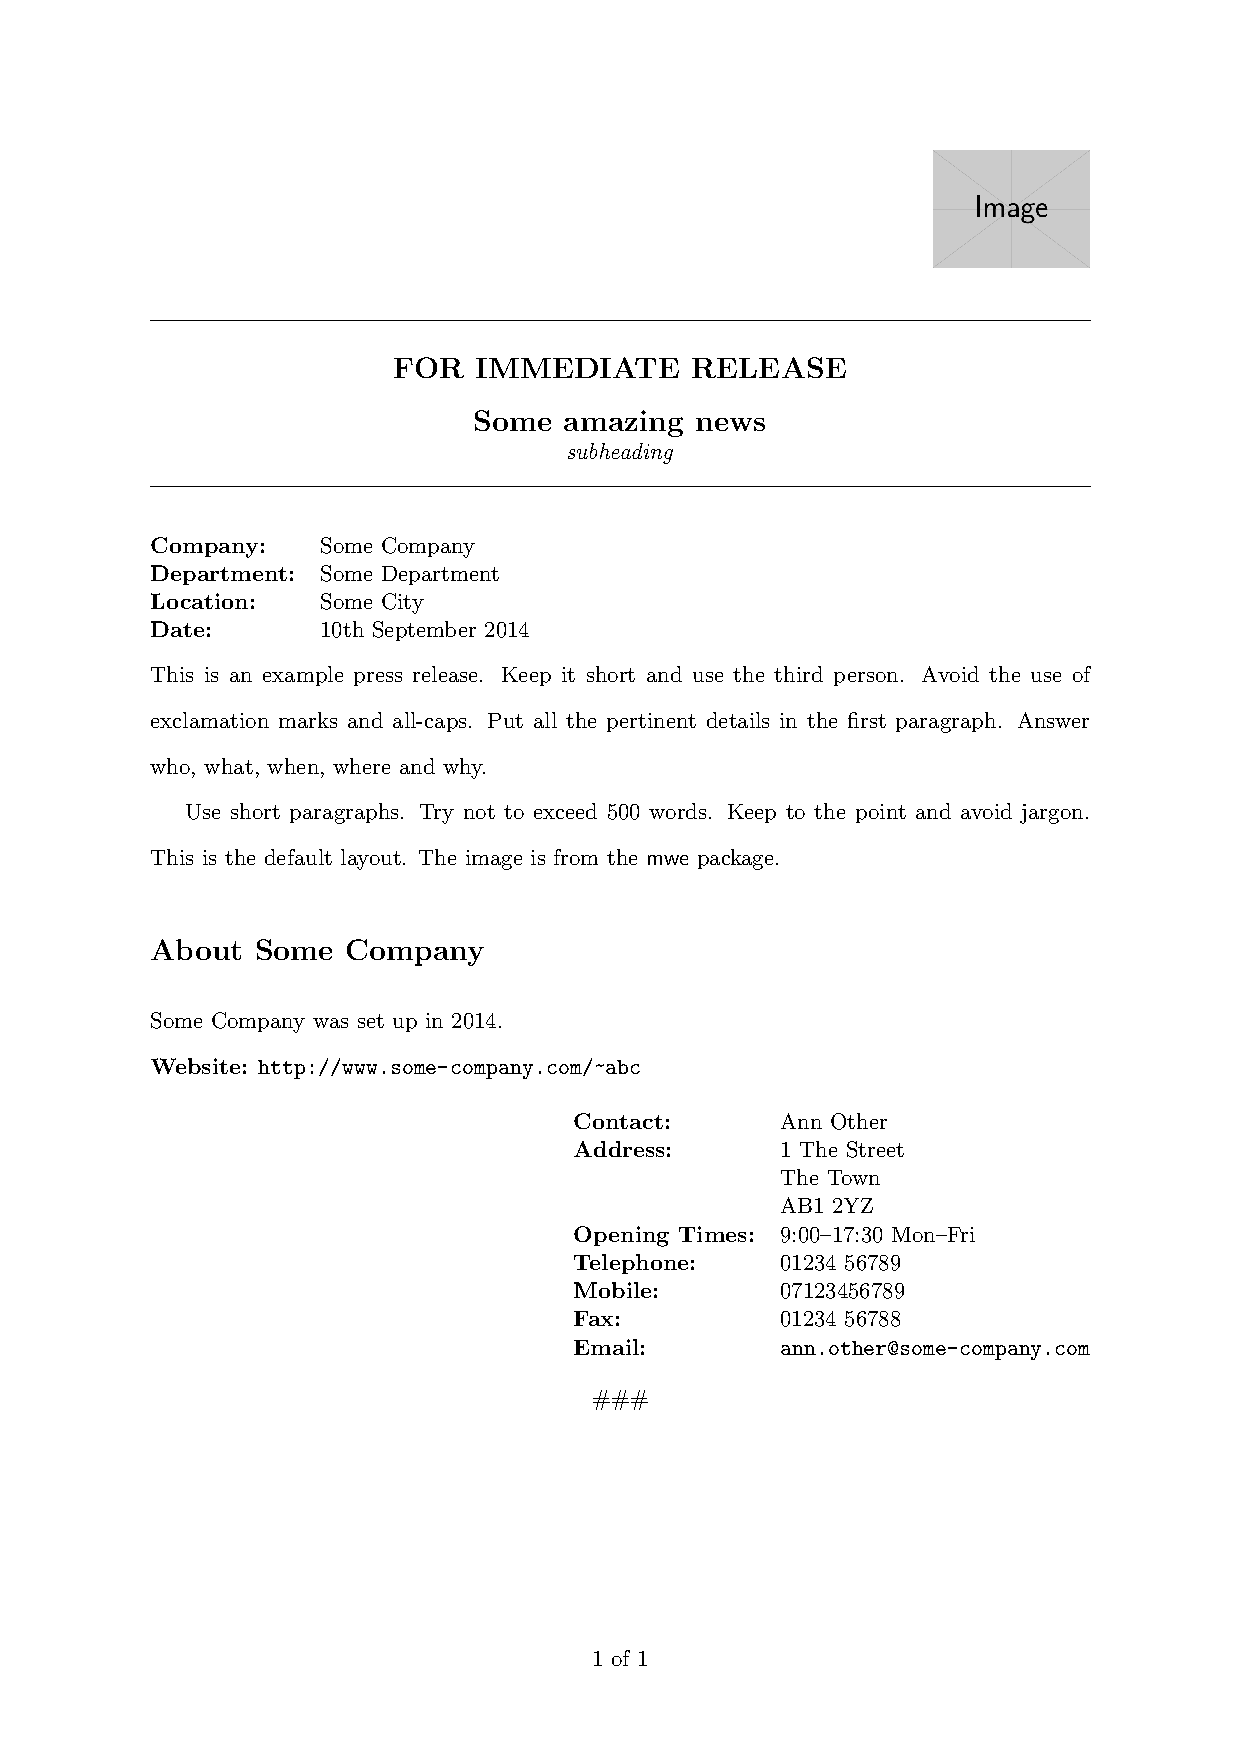
\includegraphics[height=0.9\textheight]{samples/sample-pressrelease}}
% \caption{Sample Document}
% \label{fig:sample}
%\end{figure}
%
%\clearpage
%\StopEventually{\PrintIndex}
%
%
%\section{The Code}
%\iffalse
%    \begin{macrocode}
%<*pressrelease.cls>
%    \end{macrocode}
%\fi
%\subsection{pressrelease.cls}
%\changes{1.0}{2014-09-10}{Initial release}
% Declare class and required TeX format:
%    \begin{macrocode}
\NeedsTeXFormat{LaTeX2e}
\ProvidesClass{pressrelease}[2014/09/10 v1.0 (NLCT) Press Release Class]
%    \end{macrocode}
% Class options have a key=value interface.
%    \begin{macrocode}
\RequirePackage{xkeyval}
\RequirePackage{etoolbox}
%    \end{macrocode}
%
% Font size options.
%    \begin{macrocode}
\DeclareOptionX{10pt}{\PassOptionsToClass{10pt}{article}}
\DeclareOptionX{11pt}{\PassOptionsToClass{11pt}{article}}
\DeclareOptionX{12pt}{\PassOptionsToClass{12pt}{article}}
%    \end{macrocode}
% Paper size options (sizes can also be set via \cs{geometry})
%    \begin{macrocode}
\DeclareOptionX{letterpaper}{\PassOptionsToClass{letterpaper}{article}}
\DeclareOptionX{a4paper}{\PassOptionsToClass{a4paper}{article}}
%    \end{macrocode}
%
%\begin{macro}{\ifPRloadsymbols}
% Load \sty{pressrelease-symbols} if true
%    \begin{macrocode}
\define@boolkey{pressrelease.cls}[@PRload]{symbols}[true]{}
\@PRloadsymbolsfalse
%    \end{macrocode}
%\end{macro}
%
%\begin{macro}{\ifPRheadabove}
% If true, head line goes above top info block otherwise headline
% goes below top info block.
%    \begin{macrocode}
\newif\ifPRheadabove
\PRheadabovetrue
%    \end{macrocode}
%\end{macro}
%\begin{macro}{\PRheadalign}
% Headline alignment (default: centred)
%    \begin{macrocode}
\newcommand{\PRheadalign}[1]{%
 \begin{center}#1\end{center}%
}
%    \end{macrocode}
%\end{macro}
%
%    \begin{macrocode}
\define@choicekey{pressrelease.cls}{head}[\val\nr]%
 {above,below,center,left,right,centre,%
  above center,above centre,above left,above right,%
  below center,below centre,below left,below right}%
 {%
 \ifcase\nr\relax
   \PRheadabovetrue
 \or
   \PRheadabovefalse
 \or
  \renewcommand{\PRheadalign}[1]{\begin{center}##1\end{center}}%
 \or
  \renewcommand{\PRheadalign}[1]{\begin{flushleft}##1\end{flushleft}}%
 \or
  \renewcommand{\PRheadalign}[1]{\begin{flushright}##1\end{flushright}}%
 \or
  \renewcommand{\PRheadalign}[1]{\begin{center}##1\end{center}}%
 \or % above center
  \PRheadabovetrue
  \renewcommand{\PRheadalign}[1]{\begin{center}##1\end{center}}%
 \or % above centre
  \PRheadabovetrue
  \renewcommand{\PRheadalign}[1]{\begin{center}##1\end{center}}%
 \or % above left
  \PRheadabovetrue
  \renewcommand{\PRheadalign}[1]{\begin{flushleft}##1\end{flushleft}}%
 \or % above right
  \PRheadabovetrue
  \renewcommand{\PRheadalign}[1]{\begin{flushright}##1\end{flushright}}%
 \or % below centre
  \PRheadabovefalse
  \renewcommand{\PRheadalign}[1]{\begin{center}##1\end{center}}%
 \or % below center
  \PRheadabovefalse
  \renewcommand{\PRheadalign}[1]{\begin{center}##1\end{center}}%
 \or % below left
  \PRheadabovefalse
  \renewcommand{\PRheadalign}[1]{\begin{flushleft}##1\end{flushleft}}%
 \or % below right
  \PRheadabovefalse
  \renewcommand{\PRheadalign}[1]{\begin{flushright}##1\end{flushright}}%
 \fi
}
%    \end{macrocode}
%
%\begin{macro}{\PRlogoformat}
%    \begin{macrocode}
\newcommand*{\PRlogoformat}[1]{#1}
%    \end{macrocode}
% Make it possible for user to ``smash'' logo so it doesn't take up
% vertical space:
%    \begin{macrocode}
\define@choicekey{pressrelease.cls}{smashlogo}[\val\nr]{true,false}[true]{%
  \ifcase\nr\relax
    \renewcommand*{\PRlogoformat}[1]{\vbox to 0pt{##1}}%
  \or
    \renewcommand*{\PRlogoformat}[1]{##1}%
  \fi
}
%    \end{macrocode}
%\end{macro}
%
%\begin{macro}{\PRlogoalign}
%    \begin{macrocode}
\newif\ifPRlogoabove
\PRlogoabovetrue
\newcommand{\PRlogoalign}[1]{{\raggedleft\PRlogoformat{#1}\par}}
\define@choicekey{pressrelease.cls}{logo}[\val\nr]%
 {left,right,above,below,above left,above right,below left,below right}{%
  \ifcase\nr\relax
    \renewcommand{\PRlogoalign}[1]{{\raggedright\PRlogoformat{##1}\@@par}}%
  \or
    \renewcommand{\PRlogoalign}[1]{{\raggedleft\PRlogoformat{##1}\@@par}}%
  \or
    \PRlogoabovetrue
  \or
    \PRlogoabovefalse
  \or
    \PRlogoabovetrue
    \renewcommand{\PRlogoalign}[1]{{\raggedright\PRlogoformat{##1}\@@par}}%
  \or
    \PRlogoabovetrue
    \renewcommand{\PRlogoalign}[1]{{\raggedleft\PRlogoformat{##1}\@@par}}%
  \or
    \PRlogoabovefalse
    \renewcommand{\PRlogoalign}[1]{{\raggedright\PRlogoformat{##1}\@@par}}%
  \or
    \PRlogoabovefalse
    \renewcommand{\PRlogoalign}[1]{{\raggedleft\PRlogoformat{##1}\@@par}}%
  \fi
}
%    \end{macrocode}
%\end{macro}
%
%\begin{macro}{\PRreleasealign}
% Release alignment (default: centred)
%    \begin{macrocode}
\newcommand{\PRreleasealign}[1]{%
 \begin{center}#1\end{center}%
}
\define@choicekey{pressrelease.cls}{releasealign}[\val\nr]{center,left,right,centre}{%
 \ifcase\nr\relax
  \renewcommand{\PRreleasealign}[1]{\begin{center}##1\end{center}}%
 \or
  \renewcommand{\PRreleasealign}[1]{\begin{flushleft}##1\end{flushleft}}%
 \or
  \renewcommand{\PRreleasealign}[1]{\begin{flushright}##1\end{flushright}}%
 \or
  \renewcommand{\PRreleasealign}[1]{\begin{center}##1\end{center}}%
 \fi
}
%    \end{macrocode}
%\end{macro}
%
%\begin{macro}{\ifPRruled}
% Use horizontal rules if true.
%    \begin{macrocode}
\define@boolkey{pressrelease.cls}[PR]{ruled}[true]{}
\PRruledtrue
%    \end{macrocode}
%\end{macro}
%
%\begin{macro}{\PRinfotopalign}
% Contact details alignment of top info block (default: left)
%    \begin{macrocode}
\newcommand{\PRinfotopalign}[1]{%
 \begin{flushleft}#1\end{flushleft}%
}
\define@choicekey{pressrelease.cls}{topinfoalign}[\val\nr]{center,left,right,centre}{%
 \ifcase\nr\relax
  \renewcommand{\PRinfotopalign}[1]{\begin{center}##1\end{center}}%
 \or
  \renewcommand{\PRinfotopalign}[1]{\begin{flushleft}##1\end{flushleft}}%
 \or
  \renewcommand{\PRinfotopalign}[1]{\begin{flushright}##1\end{flushright}}%
 \or
  \renewcommand{\PRinfotopalign}[1]{\begin{center}##1\end{center}}%
 \fi
}
%    \end{macrocode}
%\end{macro}
%
%\begin{macro}{\PRinfobottomalign}
% Contact details alignment of bottom info block (default: right)
%    \begin{macrocode}
\newcommand{\PRinfobottomalign}[1]{%
 \begin{flushright}#1\end{flushright}%
}
\define@choicekey{pressrelease.cls}{bottominfoalign}[\val\nr]{center,left,right,centre}{%
 \ifcase\nr\relax
  \renewcommand{\PRinfobottomalign}[1]{\begin{center}##1\end{center}}%
 \or
  \renewcommand{\PRinfobottomalign}[1]{\begin{flushleft}##1\end{flushleft}}%
 \or
  \renewcommand{\PRinfobottomalign}[1]{\begin{flushright}##1\end{flushright}}%
 \or
  \renewcommand{\PRinfobottomalign}[1]{\begin{center}##1\end{center}}%
 \fi
}
%    \end{macrocode}
%\end{macro}
%
% Process options
%    \begin{macrocode}
\ProcessOptionsX
%    \end{macrocode}
% Load \cls{article} class:
%    \begin{macrocode}
\LoadClass{article}
%    \end{macrocode}
% Load required packages:
%    \begin{macrocode}
\RequirePackage{setspace}
\RequirePackage{geometry}
\RequirePackage{url}
\RequirePackage{refcount}
%    \end{macrocode}
% Set wide margins
%    \begin{macrocode}
\geometry{hmargin=1in,vmargin=1in,hcentering}
%    \end{macrocode}
% Start with single spacing.
%    \begin{macrocode}
\singlespacing
%    \end{macrocode}
%
% Text defaults:
%\begin{macro}{\PRreleasetext}
%    \begin{macrocode}
\newcommand*{\PRreleasetext}{For immediate release}
%    \end{macrocode}
%\end{macro}
%\begin{macro}{\PRcontacttext}
%    \begin{macrocode}
\newcommand*{\PRcontacttext}{Contact}
%    \end{macrocode}
%\end{macro}
%\begin{macro}{\PRphonetext}
%    \begin{macrocode}
\newcommand*{\PRphonetext}{Telephone}
%    \end{macrocode}
%\end{macro}
%\begin{macro}{\PRmobiletext}
%    \begin{macrocode}
\newcommand*{\PRmobiletext}{Mobile}
%    \end{macrocode}
%\end{macro}
%\begin{macro}{\PRemailtext}
%    \begin{macrocode}
\newcommand*{\PRemailtext}{Email}
%    \end{macrocode}
%\end{macro}
%\begin{macro}{\PRurltext}
%    \begin{macrocode}
\newcommand*{\PRurltext}{Website}
%    \end{macrocode}
%\end{macro}
%\begin{macro}{\PRfaxtext}
%    \begin{macrocode}
\newcommand*{\PRfaxtext}{Fax}
%    \end{macrocode}
%\end{macro}
%\begin{macro}{\PRcompanytext}
%    \begin{macrocode}
\newcommand*{\PRcompanytext}{Company}
%    \end{macrocode}
%\end{macro}
%\begin{macro}{\PRdepartmenttext}
%    \begin{macrocode}
\newcommand*{\PRdepartmenttext}{Department}
%    \end{macrocode}
%\end{macro}
%\begin{macro}{\PRaddresstext}
%    \begin{macrocode}
\newcommand*{\PRaddresstext}{Address}
%    \end{macrocode}
%\end{macro}
%\begin{macro}{\PRhourstext}
%    \begin{macrocode}
\newcommand*{\PRhourstext}{Opening Times}
%    \end{macrocode}
%\end{macro}
%\begin{macro}{\PRdatetext}
%    \begin{macrocode}
\newcommand*{\PRdatetext}{Date}
%    \end{macrocode}
%\end{macro}
%\begin{macro}{\PRlocationtext}
%    \begin{macrocode}
\newcommand*{\PRlocationtext}{Location}
%    \end{macrocode}
%\end{macro}
%
%\begin{macro}{\PRabouttext}
%    \begin{macrocode}
\newcommand*{\PRabouttext}{About \PRusevar{company}}
%    \end{macrocode}
%\end{macro}
%
%\begin{macro}{\PRencltext}
%    \begin{macrocode}
\newcommand*{\PRencltext}{Encl.}
%    \end{macrocode}
%\end{macro}
%
%\begin{macro}{\PRrelease}
% Set the release text.
%    \begin{macrocode}
\newcommand*{\PRrelease}[1]{\renewcommand*{\@PRrelease}{#1}}
\newcommand*{\@PRrelease}{\PRreleasetext}
%    \end{macrocode}
%\end{macro}
%
%\begin{macro}{\PRreleaseformat}
% Format used for the release text.
%    \begin{macrocode}
\newcommand*{\PRreleaseformat}[1]{\textbf{\Large\MakeUppercase{#1}}}
%    \end{macrocode}
%\end{macro}
%
%\begin{macro}{\PRdohrule}
% Do a horizontal rule if the ruled option has been set.
%    \begin{macrocode}
\newcommand{\PRdohrule}{\ifPRruled\par\noindent\hrulefill\par\noindent\fi}
%    \end{macrocode}
%\end{macro}
%
%\begin{macro}{\PRtagformat}
% Font for the tags:
%    \begin{macrocode}
\newcommand*{\PRtagformat}[1]{\textbf{#1:}}
%    \end{macrocode}
%\end{macro}
%
%\begin{macro}{\PRcompany}
% Set the company name.
%    \begin{macrocode}
\newcommand*{\PRcompany}[1]{\renewcommand*{\@PRcompany}{#1}}
\newcommand*{\@PRcompany}{}
%    \end{macrocode}
%\end{macro}
%\begin{macro}{\PRdepartment}
% Set the department name.
%    \begin{macrocode}
\newcommand*{\PRdepartment}[1]{\renewcommand*{\@PRdepartment}{#1}}
\newcommand*{\@PRdepartment}{}
%    \end{macrocode}
%\end{macro}
%\begin{macro}{\PRcontact}
% Set the contact name.
%    \begin{macrocode}
\newcommand*{\PRcontact}[1]{\renewcommand*{\@PRcontact}{#1}}
\newcommand*{\@PRcontact}{}
%    \end{macrocode}
%\end{macro}
%\begin{macro}{\PRaddress}
% Set the address.
%    \begin{macrocode}
\newcommand*{\PRaddress}[1]{\renewcommand*{\@PRaddress}{#1}}
\newcommand*{\@PRaddress}{}
%    \end{macrocode}
%\end{macro}
%\begin{macro}{\PRlocation}
% Set the location.
%    \begin{macrocode}
\newcommand*{\PRlocation}[1]{\renewcommand*{\@PRlocation}{#1}}
\newcommand*{\@PRlocation}{}
%    \end{macrocode}
%\end{macro}
%
%\begin{macro}{\PRphone}
% Set the phone number.
%    \begin{macrocode}
\newcommand*{\PRphone}[1]{\renewcommand*{\@PRphone}{#1}}
\newcommand*{\@PRphone}{}
%    \end{macrocode}
%\end{macro}
%\begin{macro}{\PRmobile}
% Set the mobile number.
%    \begin{macrocode}
\newcommand*{\PRmobile}[1]{\renewcommand*{\@PRmobile}{#1}}
\newcommand*{\@PRmobile}{}
%    \end{macrocode}
%\end{macro}
%\begin{macro}{\PRfax}
% Set the fax number.
%    \begin{macrocode}
\newcommand*{\PRfax}[1]{\renewcommand*{\@PRfax}{#1}}
\newcommand*{\@PRfax}{}
%    \end{macrocode}
%\end{macro}
%
%\begin{macro}{\PRemail}
% Set the email address.
%    \begin{macrocode}
\newcommand*{\PRemail}[1]{\renewcommand*{\@PRemail}{\PRemailformat{#1}}}
\newcommand*{\@PRemail}{}
%    \end{macrocode}
%\end{macro}
%
%\begin{macro}{\PRemailformat}
%    \begin{macrocode}
\newcommand*{\PRemailformat}[1]{\texttt{#1}}
%    \end{macrocode}
%\end{macro}
%
%\begin{macro}{\PRurl}
% Set the web address.
%    \begin{macrocode}
\newcommand*{\PRurl}[1]{\renewcommand*{\@PRurl}{\protect\url{#1}}}
\newcommand*{\@PRurl}{}
%    \end{macrocode}
%\end{macro}
%
%\begin{macro}{\PRhours}
% Set the opening hours.
%    \begin{macrocode}
\newcommand*{\PRhours}[1]{\renewcommand*{\@PRhours}{#1}}
\newcommand*{\@PRhours}{}
%    \end{macrocode}
%\end{macro}
%
%\begin{macro}{\PRlogo}
% Set the company logo.
%    \begin{macrocode}
\newcommand*{\PRlogo}[1]{\renewcommand*{\@PRlogo}{#1}}
\newcommand*{\@PRlogo}{}
%    \end{macrocode}
%\end{macro}
%
%\begin{macro}{\PRencl}
% Set the enclosure text.
%    \begin{macrocode}
\newcommand*{\PRencl}[1]{\renewcommand*{\@PRencl}{#1}}
\newcommand*{\@PRencl}{}
%    \end{macrocode}
%\end{macro}
%
%\begin{macro}{\PRusevar}
% Access information set using the above commands.
%    \begin{macrocode}
\newcommand*{\PRusevar}[1]{\csuse{@PR#1}}
%    \end{macrocode}
%\end{macro}
% Allow the date to be accessed in the same way.
%    \begin{macrocode}
\newcommand*{\@PRdate}{\@date}
%    \end{macrocode}
%
%\begin{macro}{\PRinfotopblock}
%\begin{definition}
%\cs{PRinfotopblock}\marg{company}\marg{department}\marg{location}\marg{contact
%name}\marg{address}\marg{opening
%hours}\marg{phone}\marg{email}\marg{date}
%\end{definition}
% Order of information in the top info block.
%    \begin{macrocode}
\newcommand{\PRinfotopblock}[9]{#1#2#3#9}
%    \end{macrocode}
%
%\begin{macro}{\PRinfobottomblock}
%\begin{definition}
%\cs{PRinfobottomblock}\marg{company}\marg{department}\marg{location}\marg{contact
%name}\marg{address}\marg{opening
%hours}\marg{phone}\marg{email}\marg{date}
%\end{definition}
% Order of information in the bottom info block.
%    \begin{macrocode}
\newcommand{\PRinfobottomblock}[9]{#4#5#6#7#8}
%    \end{macrocode}
%
% Provide option to set order of items in the info blocks. First define a list parser that
% uses the hyphen character as the separator.
%    \begin{macrocode}
\DeclareListParser*{\@PR@forslashlist}{/}
\newcommand*{\@PR@slashlistdo}[1]{%
  \ifstrequal{#1}{company}%
  {\appto\@PR@infoargs{##1}}%
  {%
    \ifstrequal{#1}{department}%
    {\appto\@PR@infoargs{##2}}%
    {%
      \ifstrequal{#1}{location}%
      {\appto\@PR@infoargs{##3}}%
      {%
        \ifstrequal{#1}{contact}%
        {\appto\@PR@infoargs{##4}}%
        {%
          \ifstrequal{#1}{address}%
          {\appto\@PR@infoargs{##5}}%
          {%
            \ifstrequal{#1}{hours}%
            {\appto\@PR@infoargs{##6}}%
            {%
              \ifstrequal{#1}{phone}%
              {\appto\@PR@infoargs{##7}}%
              {%
                \ifstrequal{#1}{email}%
                {\appto\@PR@infoargs{##8}}%
                {%
                  \ifstrequal{#1}{date}%
                  {\appto\@PR@infoargs{##9}}%
                  {%
                    \ClassError{pressrelease}%
                    {Unknown info block option `#1'}%
                    {Available options: `company', `department',
                    `location', `contact', `address', `hours', `phone',
                    `email', `date'}%
                  }%
                }%
              }%
            }%
          }%
        }%
      }%
    }%
  }%
}
%    \end{macrocode}
%
% The options below can't be passed as class options. They must be
% set using \cs{PRset}.
%
%    \begin{macrocode}
\define@key{pressrelease.cls}{topinfo}{%
    \def\@PR@infoargs{}%
    \@PR@forslashlist\@PR@slashlistdo{#1}%
    \expandafter\renewcommand\expandafter\PRinfotopblock
     \expandafter[\expandafter9\expandafter]\expandafter{\@PR@infoargs}%
}
%    \end{macrocode}
%\end{macro}
%
%    \begin{macrocode}
\define@key{pressrelease.cls}{bottominfo}{%
    \def\@PR@infoargs{}%
    \@PR@forslashlist\@PR@slashlistdo{#1}%
    \expandafter\renewcommand\expandafter\PRinfobottomblock
     \expandafter[\expandafter9\expandafter]\expandafter{\@PR@infoargs}%
}
%    \end{macrocode}
%\end{macro}

%\begin{macro}{\PRset}
%    \begin{macrocode}
\newcommand*{\PRset}[1]{\setkeys{pressrelease.cls}{#1}}
%    \end{macrocode}
%\end{macro}
%
%\begin{macro}{\PR@infotopline}
% Check for empty entry.
%    \begin{macrocode}
\newcommand*{\PR@infotopline}[2]{%
  \ifdefempty{#2}{}{\PRinfotopline{#1}{#2}}%
}
%    \end{macrocode}
%\end{macro}
%
%\begin{macro}{\PR@infobottomline}
% Check for empty entry.
%    \begin{macrocode}
\newcommand*{\PR@infobottomline}[2]{%
  \ifdefempty{#2}{}{\PRinfobottomline{#1}{#2}}%
}
%    \end{macrocode}
%\end{macro}
%
%\begin{macro}{\PR@doinfotop}
% Do the top info block details.
%    \begin{macrocode}
\newcommand{\PR@doinfotop}{%
  \PRinfotopalign{%
    \PR@doinfoblock\PR@infotopline\PRinfotopblock
       \PRinfotopbeginhook\PRinfotopendhook
  }%
}
%    \end{macrocode}
%\end{macro}
%
%\begin{macro}{\PR@doinfobottom}
% Do the bottom info block details.
%    \begin{macrocode}
\newcommand{\PR@doinfobottom}{%
  \PRinfobottomalign{%
    \PR@doinfoblock\PR@infobottomline\PRinfobottomblock
       \PRinfobottombeginhook\PRinfobottomendhook
  }%
}
%    \end{macrocode}
%\end{macro}
%
%\begin{macro}{\PR@doinfoblock}
%\begin{definition}
%\cs{PR@doinfoblock}\marg{info line cs}\marg{block order cs}\marg{begin hook cs}\marg{end hook cs}
%\end{definition}
% Do info block details.
%    \begin{macrocode}
\newcommand{\PR@doinfoblock}[4]{%
  \begin{tabular}{@{}ll@{}}%
    #3%
    #2%
    {%
      #1{\PRcompanytext}{\@PRcompany}%
    }%
    {%
      #1{\PRdepartmenttext}{\@PRdepartment}%
    }%
    {%
      #1{\PRlocationtext}{\@PRlocation}%
    }%
    {%
      #1{\PRcontacttext}{\@PRcontact}%
    }%
    {%
      #1{\PRaddresstext}{\@PRaddress}%
    }%
    {%
      #1{\PRhourstext}{\@PRhours}%
    }%
    {%
      #1{\PRphonetext}{\@PRphone}%
      #1{\PRmobiletext}{\@PRmobile}%
      #1{\PRfaxtext}{\@PRfax}%
    }%
    {%
      #1{\PRemailtext}{\@PRemail}%
    }%
    {%
      #1{\PRdatetext}{\@date}%
    }%
  #4%
  \end{tabular}%
}
%    \end{macrocode}
%\end{macro}
%
%\begin{macro}{\PRinfoentry}
% Format the entry information within the info line (not the tag).
%    \begin{macrocode}
\newcommand*{\PRinfoentry}[1]{\begin{tabular}[t]{@{}l@{}}#1\end{tabular}}
%    \end{macrocode}
%\end{macro}
%
%\begin{macro}{\PRinfoline}
% Generic line format for info block.
%    \begin{macrocode}
\newcommand*{\PRinfoline}[2]{%
  \PRtagformat{#1} & \PRinfoentry{#2}\tabularnewline
}
%    \end{macrocode}
%\end{macro}
%
%\begin{macro}{\PRinfotopline}
% Format line in the top info block.
%    \begin{macrocode}
\newcommand*{\PRinfotopline}{\PRinfoline}
%    \end{macrocode}
%\end{macro}
%
%\begin{macro}{\PRinfobottomline}
% Format line in the bottom info block.
%    \begin{macrocode}
\newcommand*{\PRinfobottomline}{\PRinfoline}
%    \end{macrocode}
%\end{macro}
%
%\begin{macro}{\PRinfotopbeginhook}
% Hook for user to provide additional information at the start of the
% top info block.
%    \begin{macrocode}
\newcommand*{\PRinfotopbeginhook}{}
%    \end{macrocode}
%\end{macro}
%\begin{macro}{\PRinfotopendhook}
% Hook for user to provide additional information at the end of the
% info block.
%    \begin{macrocode}
\newcommand*{\PRinfotopendhook}{}
%    \end{macrocode}
%\end{macro}
%
%\begin{macro}{\PRinfobottombeginhook}
% Hook for user to provide additional information at the start of the
% bottom info block.
%    \begin{macrocode}
\newcommand*{\PRinfobottombeginhook}{}
%    \end{macrocode}
%\end{macro}
%\begin{macro}{\PRinfobottomendhook}
% Hook for user to provide additional information at the end of the
% info block.
%    \begin{macrocode}
\newcommand*{\PRinfobottomendhook}{}
%    \end{macrocode}
%\end{macro}


%\begin{macro}{\PRheadline}
%    \begin{macrocode}
\newcommand*{\PRheadline}[1]{\renewcommand*{\@PRheadline}{#1}}
\newcommand*{\@PRheadline}{}
%    \end{macrocode}
%\end{macro}
%\begin{macro}{\PRsubheadline}
%    \begin{macrocode}
\newcommand*{\PRsubheadline}[1]{\renewcommand*{\@PRsubheadline}{#1}}
\newcommand*{\@PRsubheadline}{}
%    \end{macrocode}
%\end{macro}
%
%\begin{macro}{\PRheadformat}
%    \begin{macrocode}
\newcommand*{\PRheadformat}[1]{\textbf{\Large #1}}
%    \end{macrocode}
%\end{macro}
%\begin{macro}{\PRsubheadformat}
%    \begin{macrocode}
\newcommand*{\PRsubheadformat}[1]{\textit{#1}}
%    \end{macrocode}
%\end{macro}
%
% Just in case anyone wants to have multiple statements in a single
% document:
%    \begin{macrocode}
\newcounter{pressrelease}
%    \end{macrocode}
%
%\begin{macro}{\PRthelastpage}
%    \begin{macrocode}
\newcommand*{\PRthelastpage}{0}
%    \end{macrocode}
%\end{macro}
%
%\begin{environment}{pressrelease}
%    \begin{macrocode}
\newenvironment{pressrelease}%
{%
  \refstepcounter{pressrelease}%
  \refused{pressreleaseend.\number\c@pressrelease}%
  \xdef\PRthelastpage{%
    \getpagerefnumber{pressreleaseend.\number\c@pressrelease}}%
  \pagestyle{pressrelease}%
  \ifPRlogoabove
    \ifdefempty\@PRlogo{}{\PRlogoalign{\@PRlogo}}%
  \fi
    \PRreleasealign{%
      \PRdohrule\mbox{}\par\noindent
      \PRreleaseformat{\@PRrelease}%
      \ifPRheadabove\else\PRdohrule\fi
    }%
  \ifPRlogoabove
  \else
    \ifdefempty\@PRlogo{}{\PRlogoalign{\@PRlogo}}%
  \fi
  \ifPRheadabove
    \PRheadalign
    {%
       \PRheadformat{\@PRheadline}%
       \ifdefempty\@PRsubheadline
       {}%
       {\par\PRsubheadformat{\@PRsubheadline}}%
      \PRdohrule
    }%
    \par\noindent\PR@doinfotop
  \else
    \par\noindent\PR@doinfotop
    \PRheadalign
    {%
      \PRdohrule\mbox{}\par\noindent
       \PRheadformat{\@PRheadline}%
       \ifdefempty\@PRsubheadline
       {}%
       {\par\PRsubheadformat{\@PRsubheadline}}%
      \PRdohrule
    }%
  \fi
  \par
  \doublespacing
  \@afterheading\@afterindentfalse
}%
{%
  \par\singlespacing
  \PR@doinfobottom
  \ifdefempty{\@PRencl}{}%
  {\par\noindent\PRenclformat{\PRencltext}{\@PRencl}}%
  \PRformatendsignal{\PRendsignal}%
  \label{pressreleaseend.\number\c@pressrelease}%
}%
%    \end{macrocode}
%\end{environment}
%
%\begin{macro}{\PRenclformat}
%    \begin{macrocode}
\newcommand*{\PRenclformat}[2]{%
 \begin{tabular}{@{}ll}%
 \PRtagformat{#1}&\PRinfoentry{#2}%
 \end{tabular}}
%    \end{macrocode}
%\end{macro}
%
%\begin{macro}{\PRheaderfont}
% Font used in page header.
%    \begin{macrocode}
\newcommand*{\PRheaderfont}[1]{\textit{#1}}
%    \end{macrocode}
%\end{macro}
%
%\begin{macro}{\ps@pressrelease}
% Press release page style.
%    \begin{macrocode}
\newcommand*{\ps@pressrelease}{%
  \gdef\@oddhead{\hfill\ifnum\c@page>1\relax
    \PRheaderfont{\PRusevar{headline}}%
  \fi\hfill}%
  \global\let\@evenhead\@oddhead
  \gdef\@oddfoot{%
   \hfill
   \PRnOfm{\thepage}{\PRthelastpage}%
   \hfill}%
  \global\let\@evenfoot\@oddfoot
}
%    \end{macrocode}
%\end{macro}
%
%\begin{macro}{\PRnOfm}
%    \begin{macrocode}
\newcommand*{\PRnOfm}[2]{#1 of #2}
%    \end{macrocode}
%\end{macro}
%
%\begin{macro}{\PRendsignal}
% End of statement marker.
%    \begin{macrocode}
\newcommand*{\PRendsignal}{\#\#\#}
%    \end{macrocode}
%\end{macro}
%
%\begin{macro}{\PRformatendsignal}
%    \begin{macrocode}
\newcommand*{\PRformatendsignal}[1]{\begin{center}#1\end{center}}
%    \end{macrocode}
%\end{macro}
%
%\begin{environment}{about}
%    \begin{macrocode}
\newenvironment{about}%
 {%
  \section*{\PRabouttext}%
 }%
 {% 
   \ifdefempty\@PRurl
   {}%
   {%
     \PRurlformat{\PRurltext}{\@PRurl}\PRaboutposturlhook\par
   }%
 }
%    \end{macrocode}
%\end{environment}
%
%\begin{macro}{\PRurlformat}
%    \begin{macrocode}
\newcommand{\PRurlformat}[2]{%
  \par\noindent\PRtagformat{#1} #2}
%    \end{macrocode}
%\end{macro}
%
%\begin{macro}{\PRaboutposturlhook}
% Allow user to add text after the website address.
%    \begin{macrocode}
\newcommand*{\PRaboutposturlhook}{}
%    \end{macrocode}
%\end{macro}
%
% Finally, load \sty{pressrelease-symbols} if required:
%    \begin{macrocode}
\if@PRloadsymbols
  \RequirePackage{pressrelease-symbols}
\fi
\disable@keys{pressrelease.cls}{symbols}
%    \end{macrocode}
%\iffalse
%    \begin{macrocode}
%</pressrelease.cls>
%    \end{macrocode}
%\fi
%\iffalse
%    \begin{macrocode}
%<*pressrelease-symbols.sty>
%    \end{macrocode}
%\fi
%\subsection{pressrelease-symbols.sty}
% This package loads \sty{marvosym} and \sty{tikz} to define symbols
% for the bottom info block. The tags are suppressed for the top
% info block. This package should be used with the
% \clsfmt{pressrelease} class.
%    \begin{macrocode}
\NeedsTeXFormat{LaTeX2e}
\ProvidesPackage{pressrelease-symbols}[2014/09/10 v1.0 (NLCT)]
%    \end{macrocode}
% Load \sty{marvosym} and \sty{tikz}:
%    \begin{macrocode}
\RequirePackage{marvosym}
\RequirePackage{tikz}
%    \end{macrocode}
% Define a command to produce a paper clip symbol.
%    \begin{macrocode}
\newcommand*{\paperclip}{%
  
\begin{tikzpicture}[x=0.055ex,y=0.055ex,rotate=-90]
  \draw[line width=0.05ex] (9,-1) -- (26,-1)
   .. controls (33,1) and (33,9) ..
    (26,11) -- (8,11)
   .. controls (0,11) and (0,2) ..
     (8,2) -- (22,2)
   .. controls (26,2) and (26,8) ..
   (22,8) -- (8,8);
  \end{tikzpicture}%
}
%    \end{macrocode}
% Remove tags from top info block
%    \begin{macrocode}
\renewcommand*{\PRinfotopline}[2]{%
  \PRinfoentry{#2}\tabularnewline
}
%    \end{macrocode}
% Change textual tags to use symbols    
%    \begin{macrocode}
\renewcommand*{\PRcontacttext}{\Info}
\renewcommand*{\PRphonetext}{\Telefon}
\renewcommand*{\PRmobiletext}{\Mobilefone}
\renewcommand*{\PRfaxtext}{\fax}
\renewcommand*{\PRemailtext}{\Email}
\renewcommand*{\PRaddresstext}{\Letter}
\renewcommand*{\PRhourstext}{\ClockLogo}
\renewcommand*{\PRurltext}{\ComputerMouse}
\renewcommand*{\PRencltext}{\paperclip}
%    \end{macrocode}
% Remove the colon and bold formatting from the tag:
%    \begin{macrocode}
\renewcommand*{\PRtagformat}[1]{#1}
%    \end{macrocode}
%\iffalse
%    \begin{macrocode}
%</pressrelease-symbols.sty>
%    \end{macrocode}
%\fi
%\Finale
\endinput
